\section{Template and Data Mapping Directives}

\subsection{{\tt template} Directive}

\subsubsection*{Synopsis}

The {\tt \Directive{template}} directive declares a template. 

\subsubsection*{Syntax}
\Syntax{template}

\begin{tabular}{ll}
\verb![F]! & \verb|!$xmp template| {\it template-decl} {\openb}, {\it
 template-decl} {\closeb}... \\
& \\
\verb![C]! & \verb|#pragma xmp template| {\it template-decl} {\openb},
     {\it template-decl} {\closeb}... \\
\end{tabular}

%\begin{tabular}{ll}
%\verb![F]! & \verb|!$xmp template| {\it template-name} \verb|(| {\it template-spec} 
%{\openb}, {\it template-spec} {\closeb}... \verb|)| \\
%& \\
%\verb![C]! & \verb|#pragma xmp template| {\it template-name} \verb|(| {\it template-spec} 
%{\openb}, {\it template-spec} {\closeb}... \verb|)| \\
%\end{tabular}

\vspace{0.3cm}

where {\it template-decl} is:

\vspace{0.3cm}

\begin{tabular}{ll}
 \hspace{0.5cm} & {\it template-name} \verb|(| {\it template-spec}
 {\openb}, {\it template-spec} {\closeb}... \verb|)|
\end{tabular}

\vspace{0.3cm}

and {\it template-spec} must be one of:

\vspace{0.3cm}

\begin{tabular}{ll}
 \hspace{0.5cm} & {\openb}{\it int-expr} {\tt :}{\closeb} {\it int-expr} \\
 \hspace{0.5cm} & {\tt :} \\
\end{tabular}

\subsubsection*{Description}

The {\tt template} directive declares a template with the shape specified by
the sequence of {\it template-spec}'s. If every {\it template-spec} is
``:'', then the shape of the template is initially undefined. This
template must not be referenced until the shape is defined by {\tt
template\_fix} directives (see section \ref{subsec:template_fix
directive}) at runtime. If {\it int-expr} is specified as {\it
template-spec}, then the default lower bound is 1.

\subsubsection*{Restrictions}

\begin{itemize}
\item {\it template-name} must not conflict with any other local name in
      the same scoping unit.
\item Every {\it template-spec} must be either {\openb}{\it int-expr}
      {\tt :}{\closeb} {\it int-expr} or ``:''.
\end{itemize}


\subsection{Template Reference}

\subsubsection*{Synopsis}

The \Term{template reference} expression specified in the {\tt on} or
the {\tt from} clause of some directives is used to indirectly specify a
node set.

%The \Term{template reference} expression is used to reference a subset of
%the referenced template.

\subsubsection*{Syntax}
\Syntax{template reference}

\begin{center}
\begin{tabular}{lll}
{\it template-ref} & {\bf is} & {\it template-name} {\openb}\verb|(|
 {\it template-subscript} {\openb}, {\it
 template-subscript}{\closeb}... \verb|)|{\closeb} \\
%{\it template-subscript} & {\bf is} & {\it int-expr} $\vert$ {\it
%	 triplet} $\vert$ {\tt *} \\
\end{tabular}
\end{center}
%
\vspace{0.3cm}
%
where {\it template-subscript} must be one of:

\hspace{\hsize}

\begin{tabular}{ll}
 \hspace{0.5cm} & {\it int-expr} \\
 \hspace{0.5cm} & {\it triplet} \\
 \hspace{0.5cm} & {\tt *} \\
\end{tabular}


\subsubsection*{Description}

Being specified in the {\tt on} or the {\tt from} clause of some
directives, the template reference refers to a subset of a node set
where the specified subset of the template resides.
%The template reference refers to a subarray of the template array.  

Specifically, the ``{\tt *}'' symbol appeared as {\it
template-subscript} in a dimension of {\it template-ref} is interpreted
by each node at runtime as the indices of the elements in the dimension
that reside in the node. ``{\tt *}'' in the template reference is
equivalent to ``{\tt *}'' in the node reference.
%the position (coordinate) of each node in the dimension of the
%referenced node array.
%
%Thus, a template reference {\tt p($s_1$, ..., $s_{k-1}$, *, $s_{k+1}$, ...,
%$s_n$)} is interpreted as {\tt p($s_1$, ..., $s_{k-1}$, $j_k$,
%$s_{k+1}$, ..., $s_n$)} on the node corresponding to {\tt p($j_1$, ...,
%$j_{k-1}$, $j_k$, $j_{k+1}$, ..., $j_n$)}.

%The subscript of the subarray of a template array must be either an integer, a
%triplet, or ``{\tt *}''. The notation of the subarray using a triplet in
%the subscript is the same as that in {\Fort}. 

\subsubsection*{Examples}

Assume that {\tt t} is a template.

\begin{itemize}
\item In the {\tt task} directive, the executing node set of the task
      can be indirectly specified with a template reference in the {\tt
      on} clause.
%\item In the {\tt task} directive, a set of executing nodes is
%      indirectly specified for the task.

\Example{task}
\begin{tabular}{l}
\verb|!$xmp task on t(1:m,1:n)| \\
\verb|!$xmp task on t| \\
\end{tabular}

\item In the {\tt loop} directive, the executing node set of each
      iteration of the following loop is indirectly specified with a
      template reference in the {\tt on} clause.

\Example{loop}
\begin{tabular}{l}
\verb|!$xmp loop (i) on t(i-1)| \\
\end{tabular}%$

\item In the {\tt array} directive, the executing node set on which the
      following array assignment statement is performed in parallel is
      indirectly specified with a template reference in the {\tt on}
      clause.

\Example{array}
\begin{tabular}{l}
\verb|!$xmp array on t(1:n)| \\
\end{tabular}%$

\item In the {\tt barrier}, {\tt reduction}, and {\tt bcast} directives,
      the node set that is to perform the operation collectively can be
      indirectly specified with a template reference in the {\tt on}
      clause.

\Example{barrier}
\Example{reduction}
\begin{tabular}{l}
\verb|!$xmp barrier on t(1:n)| \\
\verb|!$xmp reduction (+:a) on t(*,:)| \\
\verb|!$xmp bcast b from p(k) on t(1:n)| \\
\end{tabular}

\end{itemize}


\subsection{{\tt distribute} Directive}

\subsubsection*{Synopsis}

The {\tt \Directive{distribute}} directive specifies the distribution of
a template.

\subsubsection*{Syntax}
\Syntax{distribute}

\begin{tabular}{ll}
\verb![F]! & \verb|!$xmp| {\tt distribute} {\it template-name} 
\verb|(|{\it dist-format} {\openb}, {\it dist-format}{\closeb}... \verb|)| {\tt onto} {\it nodes-name} \\
& \\
\verb![C]! & \verb|#pragma xmp| {\tt distribute} {\it template-name} 
\verb|(|{\it dist-format} {\openb}, {\it dist-format}{\closeb}... \verb|)| \\
& \hspace{3cm}{\tt onto} {\it nodes-name} \\
\end{tabular}
\vspace{0.3cm}

where {\it dist-format} must be one of:

\begin{tabular}{ll}
 \hspace{0.5cm} & {\tt *} \\
 & {\tt block} \\
 & {\tt cyclic} {\openb} \verb|(| {\it int-expr} \verb|)| {\closeb} \\
 & {\tt gblock} \verb|(| \{ {\tt *} $\vert$ {\it int-array} \} \verb|)| \\
\end{tabular}

\subsubsection*{Description}

According to the specified distribution format, a template is distributed
onto a specified node array. The dimension of the node array appearing in
the {\tt onto} clause corresponds, in left-to-right order, with the dimension of
the distributed template for which the corresponding {\it dist-format} is
not ``{\tt *}''. 

The interpretation of {\it dist-format} is as follows:

\begin{description}
\item[``{\tt *}'']
	   The dimension is not distributed.

\item[{\tt block}]
	   The dimension of the template is divided into
	   contiguous blocks of the same size, which are distributed onto
	   the corresponding dimension of the node array. Let {\tt d} be
	   the size of the dimension of the template, and
	   let {\tt p} be the size of the corresponding dimension of the
	   node array. If {\tt d mod p} is not zero, then the dimension
	   of the template is divided into {\tt d/ceil(d/p)} blocks of
	   size {\tt ceil(d/p)} and one block of size {\tt d\%ceil(d/p)},
	   and each block is assigned sequentially to an index along the
	   corresponding dimension of the node array. Note that if {\tt
	   k = p-d/ceil(d/p)-1 > 0}, then there is no block for the last
	   {\tt k} indices.

\item[{\tt cyclic}]
	   Equivalent to {\tt cyclic(1)}.

\item[{\tt cyclic(n)}]
	   The dimension of the template is divided into
	   contiguous blocks of size {\tt n}, and these blocks are
	   distributed onto the corresponding dimension of the node
	   array in a round-robin manner.

\item[{\tt gblock(m)}]
	   {\tt m} is referred to as a mapping array. The dimension of
	   the template is divided into contiguous blocks so that the
	   i'th block is of size {\tt m(i)}, and these blocks are
	   distributed onto the corresponding dimension of the node array.
\end{description}

If more than one {\tt gblock(*)} is specified in {\it dist-format},
then the template must not be referenced until the shape of the template
is defined by {\tt template\_fix} directives at runtime.


\subsubsection*{Restrictions}

\begin{itemize}
\item The number of {\it dist-format} that is not ``{\tt *}'' must be
      equal to the rank of the node array specified by {\it nodes-name}.  
\item The array {\it int-array} in parentheses following {\tt gblock}
      must be an integer one-dimensional array, and its size must be
      equal to the size of the corresponding dimension of the node array
      specified by {\it nodes-name}.
\item Every element of the array {\it int-array} in parentheses
      following {\tt gblock} must be a non-negative integer.
\item The sum of the elements of the array {\it int-array} in 
      parentheses following {\tt gblock} must be equal to or greater
      than the size of the corresponding dimension of the template
      specified by {\it template-name}.
\end{itemize}

\subsubsection*{Examples}
\Example{nodes}
\Example{template}
\Example{distribute}

\begin{description}
\item[Example 1]
\hspace{\hsize}
\begin{Fexample}
      program main
!$xmp nodes p(4)
!$xmp template t(64)
!$xmp distribute t(block) onto p
\end{Fexample}

The template {\tt t} is distributed in block format, as shown in the
following table.

\begin{center}
\begin{tabular}{|c|c|}
\hline
{\tt p(1)} & {\tt t(1:16)} \\
\hline
{\tt p(2)} & {\tt t(17:32)} \\
\hline
{\tt p(3)} & {\tt t(33:48)} \\
\hline
{\tt p(4)} & {\tt t(49:64)} \\
\hline
\end{tabular}
\end{center}

\item[Example 2]
\hspace{\hsize}
\begin{Fexample}
      program main
!$xmp nodes p(4)
!$xmp template t(64)
!$xmp distribute t(cyclic(8)) onto p
\end{Fexample}

The template {\tt t} is distributed in cyclic format of size eight, as
shown in the following table.

\begin{center}
\begin{tabular}{|c|c|}
\hline
{\tt p(1)} & {\tt t(1:8) t(33:40)} \\
\hline
{\tt p(2)} & {\tt t(9,16) t(41:48)} \\
\hline
{\tt p(3)} & {\tt t(17,24) t(49:56)} \\
\hline
{\tt p(4)} & {\tt t(25,32) t(57:64)} \\
\hline
\end{tabular}
\end{center}

\item[Example 3]
\hspace{\hsize}
\begin{Fexample}
      program main
!$xmp nodes p(8,5)
!$xmp template t(64,64,64)
!$xmp distribute t(*,cyclic,block) onto p
\end{Fexample}

The first dimension of the template {\tt t} is not distributed. The
second dimension is distributed onto the first dimension of the node array
{\tt p} in cyclic format. The third dimension is distributed onto the
second dimension of {\tt p} in block format. The results are as follows:

\begin{center}
\begin{tabular}{|c|c|}
\hline
{\tt p(1,1)} & {\tt t(1:64, 1:57:8, 1:13)} \\
\hline
{\tt p(2,1)} & {\tt t(1:64, 2:58:8, 1:13)} \\
\hline
... & ... \\
\hline
{\tt p(8,5)} & {\tt t(1:64, 8:64:8, 53:64)} \\
\hline
\end{tabular}
\end{center}

Note that the size of the third dimension of {\tt t} is 64 and is not
divisible by the size of the second dimension of {\tt p}. Thus, sizes of
the blocks in the third dimension are different among nodes.

\end{description}

\subsection{{\tt align} Directive}
\label{sub:align}

\subsubsection*{Synopsis}
The {\tt \Directive{align}} directive specifies that an array is to be
mapped in the same way as a specified template.

\subsubsection*{Syntax}
\Syntax{align}

\begin{tabular}{ll}
\verb![F]! & \verb|!$xmp| {\tt align} {\it array-name} \verb|(| {\it
 align-source} {\openb}, {\it align-source}{\closeb}... \verb|)| \\
 & \hspace{3cm}{\tt with} {\it template-name}
\verb|(|{\it align-subscript} {\openb}, {\it
     align-subscript}{\closeb}... \verb|)| \\ 
 & \\
\verb![C]! & \verb|#pragma xmp| {\tt align} {\it array-name} 
{\tt [}{\it align-source}{\tt ]} {\openb}{\tt [}{\it align-source}{\tt
     ]}{\closeb}... \\
 & \hspace{3cm}{\tt with} {\it template-name}
\verb|(|{\it align-subscript} {\openb}, {\it
     align-subscript}{\closeb}... \verb|)| \\
\end{tabular}
\vspace{0.3cm}

where {\it align-source} must be one of:

\vspace{0.3cm}

\begin{tabular}{ll}
 \hspace{0.5cm} & {\it scalar-int-variable} \\
 & {\tt *} \\
 & {\tt :} \\
\end{tabular}
\vspace{0.3cm}

and {\it align-subscript} must be one of:

\vspace{0.3cm}

\begin{tabular}{ll}
 \hspace{0.5cm} & {\it scalar-int-variable} {\openb} \{ {\tt +} $\vert$
 {\tt -} \} {\it int-expr} {\closeb} \\
 & {\tt *} \\
 & {\tt :} \\
\end{tabular}
\vspace{0.3cm}

Note that the variable {\it scalar-int-variable} appearing in {\it
align-source} is referred to as an ``\Term{align dummy variable}.''

\subsubsection*{Description}

The array specified by {\it array-name} is aligned with the template
specified by {\it template-name} so that each element of the array
indexed by the sequence of {\it align-source}'s is aligned with the
element of the template indexed by the sequence of {\it
align-subscript}'s, where {\it align-source}'s and {\it
align-subscript}'s are interpreted as follows:

\begin{enumerate}
\item The first form of an {\it align-source} and an {\it
      align-subscript} represents an align dummy variable and an
      expression of it, respectively. The align dummy variable ranges
      over all valid index values in the corresponding dimension of the
      array.
\item The second form ``{\tt *}'' of an {\it align-source} and an {\it
      align-subscript} represents a dummy variable (not an align dummy
      variable) that does not appear anywhere in the directive.
      \begin{itemize} 
       \item The second form of the {\it align-source} is said to
	     ``collapse'' the corresponding dimension of the array. As a
	     result, the index along the corresponding dimension makes
	     no difference in determining the alignment.
       \item The second form of the {\it align-subscript} is said to
	     ``replicate'' the array. Each element of the array is
	     replicated, and aligned to all index values in the
	     corresponding dimension of the template.
      \end{itemize}
\item The third form of an {\it align-source} and the matching {\it
      align-subscript} represents a same align dummy variable that
      ranges over all valid index values in the corresponding dimension
      of the array. The matching of colons (``{\tt :}'') in the sequence
      of {\it align-source}'s and {\it align-subscript}'s is determined
      as follows:

      \begin{itemize}
       \item \verb![F]! Colons in the sequence of {\it align-source}'s
	     and those in the sequence of {\it align-subscript}'s are
	     matched up in corresponding left-to-right order, where any
	     {\it align-source} and {\it align-subscript} that is not a
	     colon is ignored.
       \item \verb![C]! Colons in the sequence of {\it align-source}'s
	     in right-to-left order and those in the sequence of {\it 
	     align-subscript}'s in left-to-right order are matched up,
	     where any {\it align-source} and {\it align-subscript} that
	     is not a colon is ignored.
      \end{itemize}

%      If both of {\it align-source} and {\it align-subscript} is ``:'',
%      then each element of the array is aligned with each element of the
%      template.

\end{enumerate}

\subsubsection*{Restrictions}

\begin{itemize}
\item An align dummy variable may appear at most once in the sequence of
      {\it align-subscript}'s.
\item An {\it align-subscript} may contain at most one occurrence of an
      align dummy variable.
\item The {\it int-expr} in an {\it align-subscript} may not contain any
      occurrence of an align dummy variable.
\item The sequence of {\it align-sources}'s must contain exactly as many
      colons as the sequence of {\it align-subscript}'s contains.

\end{itemize}

\subsubsection*{Examples}
\Example{align}

\begin{description}
\item[Example 1]
\hspace{\hsize}
\begin{Fexample}
!$xmp align a(i) with t(i)
\end{Fexample}
%$

The array element {\tt a(i)} is aligned with the template element {\tt
t(i)}. This is equivalent to the following code.

\begin{Fexample}
!$xmp align a(:) with t(:)
\end{Fexample}
%$

\item[Example 2]
\hspace{\hsize}
\begin{Fexample}
!$xmp align a(*,j) with t(j)
\end{Fexample}
%$

The subarray {\tt a(:,j)} is aligned with the template element {\tt
t(j)}. Note that the first dimension of {\tt a} is collapsed.

\item[Example 3]
\hspace{\hsize}
\begin{Fexample}
!$xmp align a(j) with t(*,j)
\end{Fexample}
%$

The array element {\tt a(j)} is replicated, and aligned with each
template element of {\tt t(:,j)}.

\item[Example 4]
\hspace{\hsize}
\begin{Fexample}
!$xmp template t(n1,n2)
      real a(m1,m2)
!$xmp align a(*,j) with t(*,j)
\end{Fexample}
%$

	   The subarray {\tt a(:,j)} is aligned with each template
	   element of {\tt t(:,j)}.


	   By replacing ``{\tt *}'' in the first dimension of the array
	   {\tt a} and ``{\tt *}'' in the first dimension of the
	   template {\tt t} with a dummy variable {\tt i} and {\tt k},
	   respectively, this alignment can be interpreted as the
	   following mapping.

%	   If ``{\tt *}'' in the first
%	   dimension of the array {\tt a} is replaced by a dummy
%	   variable {\tt i}, and ``{\tt *}'' in the first dimension of
%	   the template {\tt t} is replaced by a dummy variable {\tt k},
%	   then we have:

$${a(i,j) \rightarrow t(k,j) \mid (i,j,k) \in (1:n1,\,1:n2,\,1:m1)}$$

\end{description}


\subsection{{\tt shadow} Directive}

\subsubsection*{Synopsis}

The {\tt \Directive{shadow}} directive declares and allocates a shadow
area for a distributed array.

\subsubsection*{Syntax}
\Syntax{shadow}

\begin{tabular}{ll}
\verb![F]! & \verb|!$xmp| {\tt shadow} {\it array-name} \verb|(| {\it
 shadow-width} {\openb}, {\it shadow-width}{\closeb}... \verb|)| \\
& \\
\verb![C]! & \verb|#pragma xmp|  {\tt shadow} {\it array-name} {\tt
     [}{\it shadow-width}{\tt ]}{\openb}{\tt [}{\it shadow-width}{\tt
     ]}{\closeb}... \\
\end{tabular}
\vspace{0.3cm}

where {\it shadow-width} must be one of:

\vspace{0.3cm}

\begin{tabular}{ll}
 \hspace{0.5cm} & {\it int-expr} \\
 & {\it int-expr} : {\it int-expr}\\
 & \verb|*|\\
\end{tabular}

\subsubsection*{Description}

The {\tt shadow} directive specifies the width of the shadow area of an
array specified by {\it array-name}, which is used to communicate the
neighbor element of the block of the array.
%
When {\it shadow-width} is of the form ``{\it int-expr} : {\it
int-expr},'' the shadow area of the width specified by the first {\it
int-expr} is added at the lower bound and that specified by the second
one at the upper bound in the dimension.
%
When {\it shadow-width} is of the form {\it int-expr}, the shadow
area of the same width specified is added at both the upper and lower
bounds in the dimension.
%
When {\it shadow-width} is of the form ``\verb|*|'', the entire area of
the array is allocated on each node, and all of the area that it does not
own is regarded as shadow.
%
This type of shadow is sometimes referred to as a ``full shadow.''

Note that the shadow area of a multi-dimensional array include
``obliquely-neighboring'' elements, which are the ones owned by the node 
whose indices are different in more than one dimension, and that the
shadow area can be allocated also at the global lower and upper bound of
an array.

The data stored in the storage area declared by the {\tt shadow}
directive is referred to as a ``\Term{shadow object}.''
%The shadow object can be
%explicitly defined and referenced only by the below-described method.
%
A shadow object represents an element of a distributed array and 
corresponds to the data object that represents the same
element as it. The corresponding data object is referred to as the
reflection source of the shadow object.

%Of the data allocated to a storage area other than a shadow area, data
%representing the same array element as that of a shadow object is called
%a reflection source of the shadow object. Conceptually, a shadow object
%and its reflection source are not mapped to one processor at the same
%time.

%A shadow
%object is not mapped to a processor to which its reflection source is
%mapped. 

\subsubsection*{Restrictions}

\begin{itemize}
\item The value specified by {\it shadow-width} must be a non-negative
      integer.
\end{itemize}

\subsubsection*{Example}
\Example{shadow}

\begin{minipage}{0.5\hsize}
\begin{center}
\begin{Fexample}
!$xmp nodes p(4,4)
!$xmp template t(64,64)
!$xmp distribute t(block,block) onto p

      real a(64,64)
!$xmp align a(i,j) with t(i,j)
!$xmp shadow a(1,1)
\end{Fexample}
\end{center}
\end{minipage}
%
\hspace{0.5cm}
%
\begin{minipage}{0.4\hsize}
\begin{figure}[H]
\begin{center}
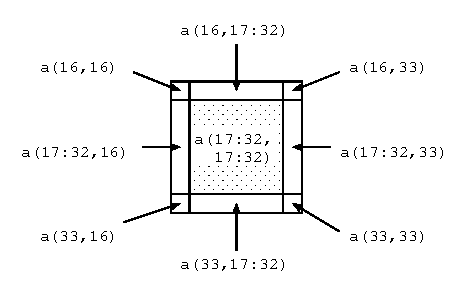
\includegraphics[width=\hsize]{figs/fig3.1.eps}
\end{center}
\caption{Example of Shadow of a Two-dimensional Array}
\label{fig3.1}
\end{figure}
\end{minipage}

\vspace{0.5cm}

The node {\tt p(2,2)} has {\tt a(17:32,17:32)} as a data object, and
{\tt a(16,16)}, {\tt a(17:32,16)}, {\tt a(33,16)}, {\tt a(16,17:32)},
{\tt a(33,17:32)}, {\tt a(16,33)}, {\tt a(17:32,33)} and {\tt a(33,33)}
as shadow objects (Figure \ref{fig3.1}). Among them, {\tt a(16,16)},
{\tt a(33,16)}, {\tt a(16,33)} and {\tt a(33,33)} are
``obliquely-neigboring'' elements of {\tt p(2,2)}.


\subsection{{\tt template\_fix} Directive}
\label{subsec:template_fix directive}

\subsubsection*{Synopsis}

This directive is an executable directive that fixes the shape and/or
the distribution of an undefined template. 

\subsubsection*{Syntax}
\Syntax{template\_fix}

\begin{tabular}{ll}
\verb![F]! & \verb|!$xmp| {\tt template\_fix} {\openb}\verb|(| {\it
 dist-format} {\openb}, {\it dist-format}{\closeb}... \verb|)|{\closeb}\\
 & \hspace{3cm}{\it template-name} {\openb}\verb|(|{\it template-spec}
 {\openb}, {\it template-spec}{\closeb}... \verb|)|{\closeb} \\
& \\
\verb![C]! & \verb|#pragma xmp|  {\tt template\_fix} {\openb}\verb|(|
     {\it dist-format} {\openb}, {\it
     dist-format}{\closeb}...\verb|)|{\closeb}\\
 & \hspace{3cm}{\it template-name} {\openb}\verb|(|{\it template-spec}
     {\openb}, {\it template-spec}{\closeb}... \verb|)|{\closeb} \\
\end{tabular}
\vspace{0.3cm}

where {\it template-spec} is:

\vspace{0.3cm}

\begin{tabular}{ll}
 \hspace{0.5cm} & {\openb}{\it int-expr} :{\closeb} {\it int-expr} \\
\end{tabular}
\vspace{0.3cm}

and {\it dist-format} is one of:

\vspace{0.3cm}

\begin{tabular}{ll}
 \hspace{0.5cm} & {\tt *} \\
 & {\tt block} \\
 & {\tt cyclic} {\openb}\verb|(| {\it int-expr} \verb|)|{\closeb} \\
 & {\tt gblock} \verb|(| {\it int-array} \verb|)| \\
\end{tabular}

\subsubsection*{Description}

The {\tt template\_fix} directive is an executable directive to fix the
shape and/or the distribution of the template that is initially
undefined, by specifying the sizes and/or the distribution format of
each dimension at runtime. The array aligned with an initially undefined
template must be an allocatable array, in {\Fort}, or a pointer (see
Section \ref{sec:Dynamic Allocation of Global Data in C}), in
{\C}, which cannot be allocated until the template is fixed by the
{\tt template\_fix} directive. Any executable directives that have such a
template in their {\tt on} clause must not be encountered until the
template is fixed by the
{\tt template\_fix} directive. Any undefined template can be fixed only
once by the {\tt template\_fix} directive in its scoping unit.

The meaning of the sequence of {\it dist-format}'s is the same
as that in the {\tt distribute} directive.

\subsubsection*{Restrictions}

\begin{itemize}
\item When a node encounters a {\tt template\_fix} directive at runtime,
      the template specified by {\it template-name} must be undefined.
\item If the sequence of {\it dist-format}'s exists in a {\tt
      template\_fix} directive, it must be identical with the 
      sequence of {\it dist-format}'s in the {\tt distribute} directive
      for the template specified by {\it template-name}, except for {\it
      int-array}, not an asterisk (``{\tt *}''), specified in the
      parenthesis following {\tt gblock}.
\item Either the sequence of {\it dist-format}'s or the sequence of {\it
      template-spec}'s must be given. 
\item The {\tt template\_fix} directive must appear in executable
      context.
\end{itemize}

\subsubsection*{Example}
\Example{template}
\Example{distribute}
\Example{align}
\Example{template\_fix}

\begin{Fexample}
!$xmp template :: t(:)
!$xmp distribute (gblock(*)) :: t

      real , allocatable :: a(:)
!$xmp align (i) with t(i) :: a
      ...
      N = ...; M(...) = ...
      ...
!$xmp template_fix(gblock(M)) t(N)
      ...
      allocate (a(N))
\end{Fexample}

Since the shape is {\tt (:)} and the distribution format is {\tt
gblock(*)}, 
the template {\tt t} is initially undefined. The allocatable array
{\tt a} is aligned to {\tt t}. After the size {\tt N} of {\tt t} and the
mapping array {\tt M} is defined, {\tt t} is fixed by the {\tt
  template\_fix} directive and {\tt a} is allocated.


%\subsection{Local Section of Mapped Data}